\documentclass[12pt]{article}
\usepackage{multirow, graphicx, tabularx, hyperref, subcaption, setspace, pgfgantt, enumitem, pgfplots}
\usepackage[margin=1.in]{geometry}
\usepackage{mathptmx}
\providecommand{\keywords}[1]
{\textbf{\textit{Keywords: }} #1}
\setlength{\parskip}{1em}

\makeatletter
\renewcommand{\section}{\@startsection {section}{1}{\z@}%
             {-3.5ex \@plus -1ex \@minus -.2ex}%
             {2.3ex \@plus .2ex}%
             {\normalfont\Large\scshape\bfseries}}

\renewcommand{\subsection}{\@startsection{subsection}{2}{\z@}%
             {-3.25ex\@plus -1ex \@minus -.2ex}%
             {1.5ex \@plus .2ex}%
             {\normalfont\large\scshape\bfseries}}

\renewcommand{\subsubsection}{\@startsection{subsubsection}{2}{\z@}%
             {-3.25ex\@plus -1ex \@minus -.2ex}%
             {1.5ex \@plus .2ex}%
             {\normalfont\normalsize\scshape\bfseries}}
\makeatother

\makeatletter
\g@addto@macro{\UrlBreaks}{\UrlOrds}
\makeatother

\renewcommand{\baselinestretch}{1.5}

\begin{document}

\begin{titlepage}

\newcommand{\HRule}{\rule{\linewidth}{0.5mm}}

\center

\textsc{\LARGE University of Abertay}\\[1.5cm]
\textsc{\Large Honours Dissertation}\\[0.5cm]

\HRule \\[0.4cm]
{ \huge \bfseries Adaptive User Interfaces For Virtual Reality}\\[0.4cm]
\HRule \\[1.5cm]

\begin{minipage}{0.4\textwidth}
\begin{flushleft} \large
\emph{Author:}\\
James \textsc{Wood}
\end{flushleft}
\end{minipage}
~
\begin{minipage}{0.4\textwidth}
\begin{flushright} \large
\emph{Supervisor:} \\
Dr. Paul \textsc{Robertson}
\end{flushright}
\end{minipage}\\[2cm]

{\large \today}\\[2cm]


\includegraphics{logo.png}\\[1cm]

\vfill

\end{titlepage}

\pagebreak

\tableofcontents
\listoffigures
\listoftables
\thispagestyle{empty}

\pagebreak

\setcounter{page}{1}

\section{Abstract}
Virtual reality allows users to interact with three-dimesional environments and interface in an intuitive way, looking around with the head mounted display and reaching out with wireless tracked controllers. Although VR interfaces often take advantage of the new space and depth afforded by the stereoscopic 3D inherent in a head mounted display, they are generally still static like the 2D interfaces prevalent on other devices.

This project expands on research made in the area of adaptive user interfaces which focused on 2D interaction, applying techniques in the 3D, motion controlled environment of VR. Adaptive user interfaces aim to improve usability with dynamic elements and input analysis. The two techniques focused on in this project are error analysis and adaptive scaling. To implement an application for evaluating these techniques C++ and Unreal Engine 4 were used.

One of the most common and difficult to use interaction models in virtual reality is the laser pointer. Interacting with far away elements can be cumbersome using a pointer and is an area in which adaptive techniques can easily be applied. As such the application used for testing during this project has the user perform simple selection and deselection interactions on a series of balls using a laser pointer to sort them in to baskets. The user testing is also timed to encourage rapid interaction and increase the number of data points.

To evaluate the benefits of the adaptive techniques applied in the application, both quantitative questionnaire data and qualitative data have been gathered and analysed. To measure the usability of the adaptive techniques the process used a static control interface. Combing the two sets of data and comparing gives a clear representation of the effect the adaptive techniques have on usability.

The results gathered show that adaptive user interface techniques... UPDATE WITH RESULTS

\keywords{Virtual Reality, User-Interfaces, 3D Interfaces, Adaptive Interfaces, Interface Plasticity}

\section{Introduction}

\subsection{The fall and rise of virtual reality}
Virtual reality (VR) head mounted displays first started appearing in the commercial market in the 1990s with Nintendo's Virtual Boy as the face of what was sold as a new era in entertainment technology. The virtual boy and its ilk failed miserably due to severe motion sickness and its utilisation of displays far worse than those available for the standard consoles at the time. Despite this rough start, two decades later VR has begun to secure its place in mainstream entertainment especially in the world of video games, although Nintendo is nowhere to be seen. 

Sony's PlayStation VR headset was more successful than predicted (Seeto 2016) and the fears surrounding the motion sickness that doomed the previous wave of VR are dissipating (Pino 2016). Alongside Sony's offering are HTC's Vive and Facebook's Oculus not mentioning the vast number of headsets designed for smartphones. These three headsets all provide similar experiences: high resolution displays for each eye providing stereoscopic depth, six degrees of freedom head tracking and hand tracking using wireless controllers. 

There have been some stand out applications and games from these early years of the new VR platforms. Job Simulator (see figure 1a) somehow turns the mundane tasks of everyday life into fun, captivating play and would not be the same experience without the head and controller tracking that comes with the HTC Vive. Tilt Brush (see figure 1b) was the first breakthrough success on the creation front with users creating thousands of sculptures using the signature 'light ribbons'. It showed that the intuitive 3D of VR could be used to great effect in productivity applications.

Even before the first release of the main VR platforms as consumer products the major Game Engine creators, Unity and Unreal Engine, had begun implementing VR support not just for applications but for the editor used to create applications. This allows not just VR developers but all developers to utilise the precision that comes with the spacial awareness to edit 3D environments with ease.

\begin{figure*}
\centering
\begin{subfigure}{.5\textwidth}
  \centering
  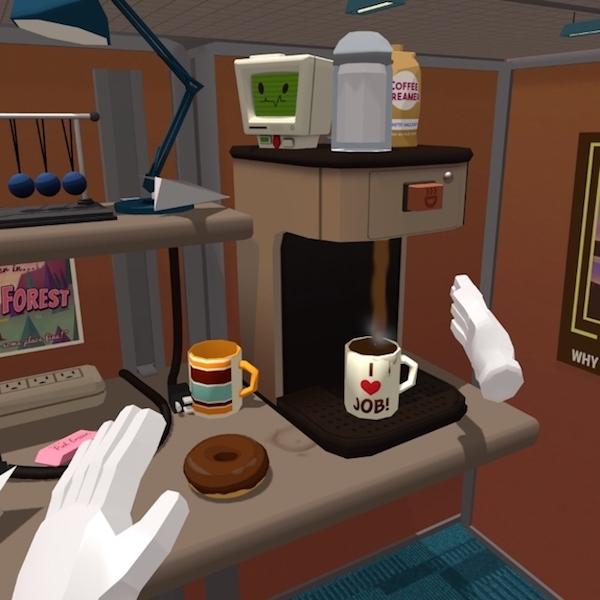
\includegraphics[width=.95\linewidth]{jobsimulator.jpg}
  \caption{Job Simulator (Owlchemy Labs 2016)}
\end{subfigure}%
\begin{subfigure}{.5\textwidth}
  \centering
  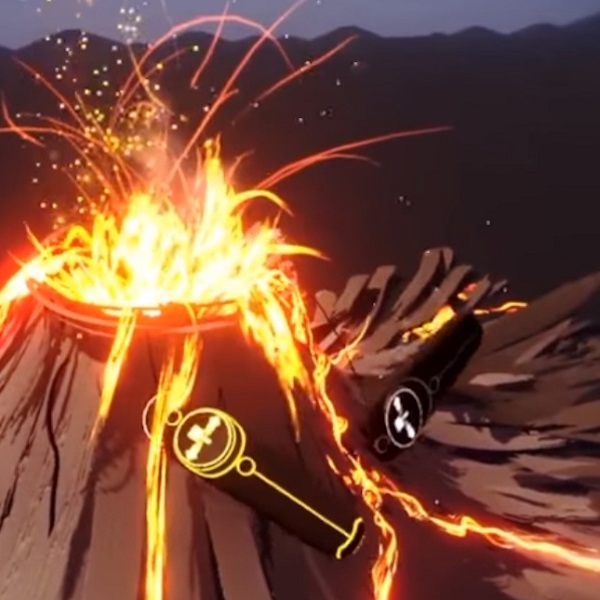
\includegraphics[width=.95\linewidth]{tiltbrush.jpg}
  \caption{Tilt Brush (Google 2016)}
\end{subfigure}
\caption{Examples of Virtual Reality applications}
\end{figure*}

\subsection{The future of immersive technologies}
The features of the forerunning virtual reality headsets combine to create a sense of immersion or 'presence' rarely achieved in traditional 2D applications and games. Even though this new wave of VR has only been around for a few years a new technology is rapidly approaching. On the horizon is the next step in immersive technology, augmented reality (AR). This will allow a wireless experience and build upon the work in mobile virtual reality by Google and Samsung. Microsoft's Hololens provides a glimpse at this future, one of seamless multi-user interaction overlaid onto reality. 

Something often associated with VR is the isolation wearing a headset implies. AR reverses this by allowing the user to still see and interact with the real world while experiencing an immersive experience. The Hololens, even in its primitive first form, demonstrates how this can introduce new forms of interaction not possible in any other way. The ability for two people to interact and collaborate with the same interface while still seeing their surroundings with no constraint on location is revolutionary.

\subsection{Interfaces in 3D}

Although everything studied and evaluated in this project can apply to any 3D interface, the testing and implementation focus on virtual reality as a platform, specifically the HTC Vive. Current virtual reality interfaces focus on interaction using the controller itself which constrains elements to being within arms reach.

A common solution is a 3D laser pointer used to select and manipulate distant elements. As in the real world using a laser pointer at a distance can be imprecise and slow (Malaika 2015) when under pressure. It is however an intuitive and unobtrusive mechanic and easily translates from the traditional desktop input of a mouse cursor.

This project evaluates how the usability of 3D interfaces in VR, specifically those utilising a 3D pointer system, can benefit from being dynamic and adaptive. It references concepts and techniques such as error analysis, adaptive scaling and user modelling explored previously by other researchers in 2D and 3D. Figure 2 shows a comparison between a traditional 2D interface and a 3D virtual reality interface.

\begin{figure*}
\centering
\begin{subfigure}{.5\textwidth}
  \centering
  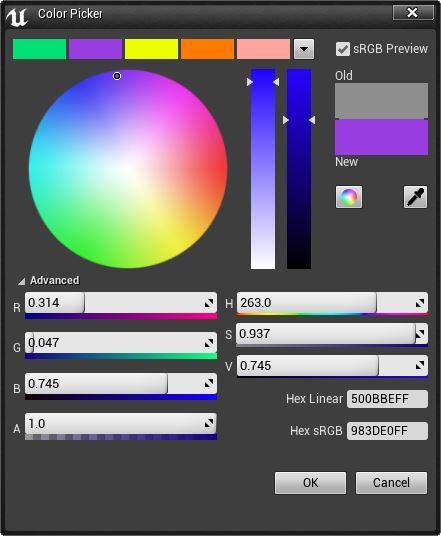
\includegraphics[width=.82\linewidth]{2dui.jpg}
  \caption{2D picker (UnrealEngine4 2012)}
\end{subfigure}%
\begin{subfigure}{.5\textwidth}
  \centering
  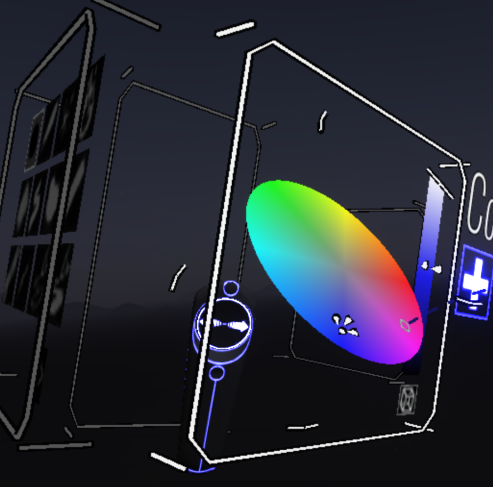
\includegraphics[width=1\linewidth]{3dui.png}
  \caption{3D colour picker (Tilt Brush 2016)}
\end{subfigure}
\caption{Comparison between 2D and 3D interface}
\end{figure*}


\subsection{Research Question} 

The project focuses on a single point: \emph{"How can the usability of virtual reality interfaces benefit from adaptive techniques?"}. In order to begin implementing the application and prepare for evaluation this research question was separated into several aims and objectives as follows:

\textbf{Aims:}
\begin{itemize}[noitemsep,topsep=0pt]
\item Apply adaptive techniques to a static virtual reality user interface.
\item Gather quantitative data through user testing and error analysis.
\item Gather qualitative data using questionnaires.
\item Evaluate the overall effect of adaptive techniques on the usability of a virtual reality interface using the data gathered.
\end{itemize}

\textbf{Objectives:}
\begin{itemize}[noitemsep,topsep=0pt]
\item Research adaptive user interface techniques for 2D and 3D interfaces.
\item Implement a 3D user interface for use in virtual reality.
\item Employ the researched techniques for assessment.
\item Create a system for error analysis to gather qualitative evaluation data.
\item Have users test the iterations of the interface and feedback on their usability.
\item Compare the various techniques using the qualitative and quantitative data gathered to evaluate their effectiveness.
\item Using the comparisons evaluate the overall impact of adaptive user interfaces on usability in virtual reality.
\end{itemize}

\section{Literature Review}
\subsection{Adaptive User Interfaces}
Dynamic user interfaces fall under a few categories in the area of research sometimes referred to as 'interface plasticity'. ‘A survey of plasticity in 3D user interfaces' (Jeremy 2014) gives an overview of the different types of dynamic user interface classifying them using two parameters, the adaptation time and the controller. Within these parameters an adaptive user interface is defined as being adapted by the system at run-time. This project focuses on implementing systems that fall under this classification of adaptation.

Many researchers have explored various ways to assist the user in digital environments since the early days of personal computing (Morgan 1998). One strategy known as intelligent user interfaces, seeks to actively learn how a user interacts with an interface and suggest or highlight relevant information accordingly. Although this can be effective, it takes time to model the user in a meaningful way and can seem obstructive as demonstrated by Microsoft's Clippy (Meyer 2015).

Another approach, the one this project focuses on, is to adapt the interface itself in direct response to the user's actions. One of these techniques covered by 'Modeling error-based Adaptive User Interfaces' (Kathik 2011) monitors the user's failures while navigating and interacting with an application to dynamically interpret their desired interaction. 'Adaptive Hypermedia and Adaptive Web-Based Systems' (Peter 2000) discusses the benefits of adapting a 3D environment as the user interacts with it to assist their actions.

Most user interfaces in our digital lives are static with adaptive interfaces reserved for improving accessibility for atypical users or use-cases. VR provides a new platform for innovation and does not have a direct counterpart to the universal language of 2D interfaces' windows and pointers. This uncharted territory provides an opportunity to experiment with dynamic 3D interfaces in new ways.

\begin{figure*}
\centering
  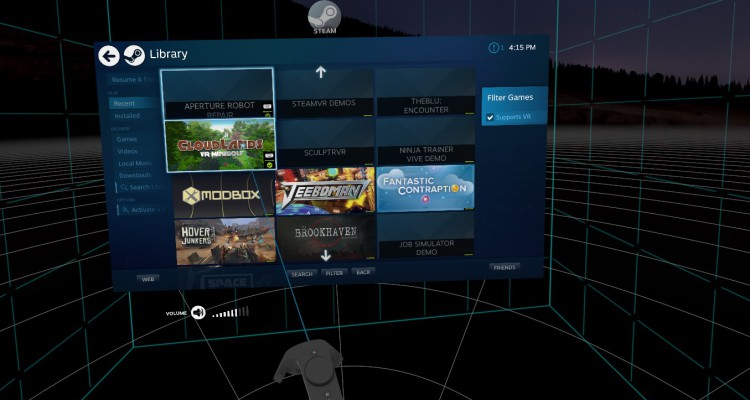
\includegraphics[width=.8\linewidth]{steamvr.jpg}
  \caption{Pointer based interaction (Steam VR 2016)}
\end{figure*}

\subsection{Virtual reality user interfaces}

When considering the current landscape of virtual reality applications and games there are a large number using motion controllers as opposed to traditional input methods such as console controllers and keyboard/mouse. The HTC Vive's lighthouse tracking system provides accurate motion control walking around a large space up to 15 ft square. The Oculus' and PSVR's use of optical tracking lends itself to a seated experience but still allows full 360 degrees of movement. 

Considering that most content on VR platforms is not exclusive to a single device experiences focus on interaction at arms length to accommodate for seated users. Interactions often consist of selecting 3D objects or interface elements by moving a controller to their position and pressing a button. Any interaction beyond arms length generally utilises a 3D pointer system as seen in the Steam VR interface (Figure 4) used to enter applications for the HTC Vive.

3D object hand-based interfaces can feel natural to use like selecting a tiny version of a level in Fantastic Contraption (see figure 3a). Having the user interact with something that is a visual representation of its function is intuitive although similar approaches in other games can be confusing. In First Contact (see figure 3b) the floppy disks used to activate various mini-games do not jump out as a vital component of the interface. Pointer interfaces are less prone to these issues as the nature of a traditional user interface is to be interacted with. As soon as the user is given a pointer and there is an element displayed it becomes a point of focus. Pointer interfaces can be brought into the context of an application to help sustain immersion as in the Brookhaven Experiment (see figure 3c) in which the user fires their gun at the menus, a similar approach is taken in Until Dawn: Rush of Blood. 

Pointer interfaces can also be far faster to use and more complex than hand-based object interfaces much in the way that a desktop cursor is often more efficient than its touch equivalent. Unfortunately these pointer interfaces become more cumbersome to use the further away, smaller and more complex they become. Despite this there are few interfaces using dynamic or adaptive elements to improve their usability. By simply assisting the user in their interaction great improvements could be made to bring VR closer to replacing desktop PCs and traditional 2D displays for everyday tasks like word processing and file management.

\begin{figure*}
\centering
\begin{subfigure}{.33\textwidth}
  \centering
  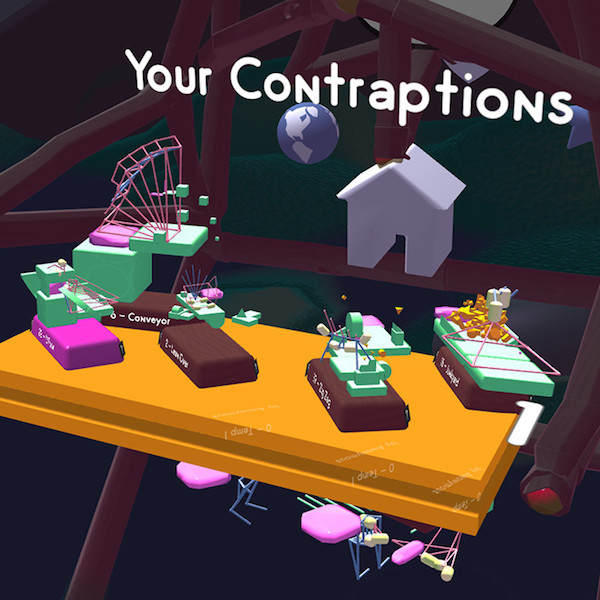
\includegraphics[width=.95\linewidth]{fantasticcontraption.jpg}
  \caption{Fantastic Contraption (2016)}
\end{subfigure}%
\begin{subfigure}{.33\textwidth}
  \centering
  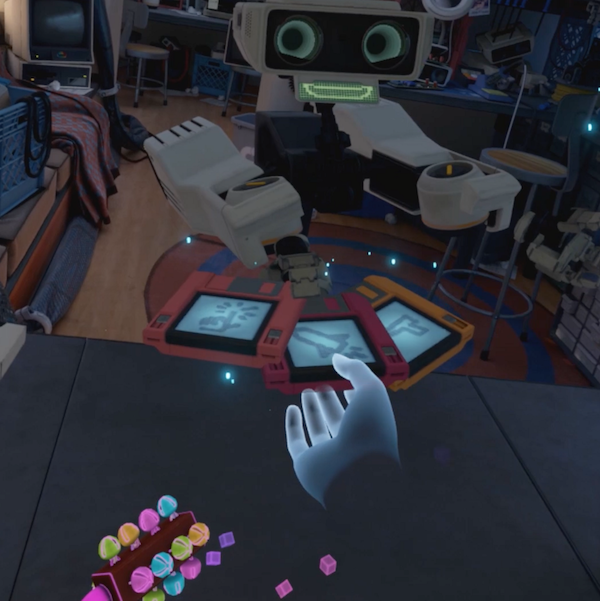
\includegraphics[width=.95\linewidth]{firstcontact.png}
  \caption{First Contact (2016)}
\end{subfigure}%
\begin{subfigure}{.33\textwidth}
  \centering
  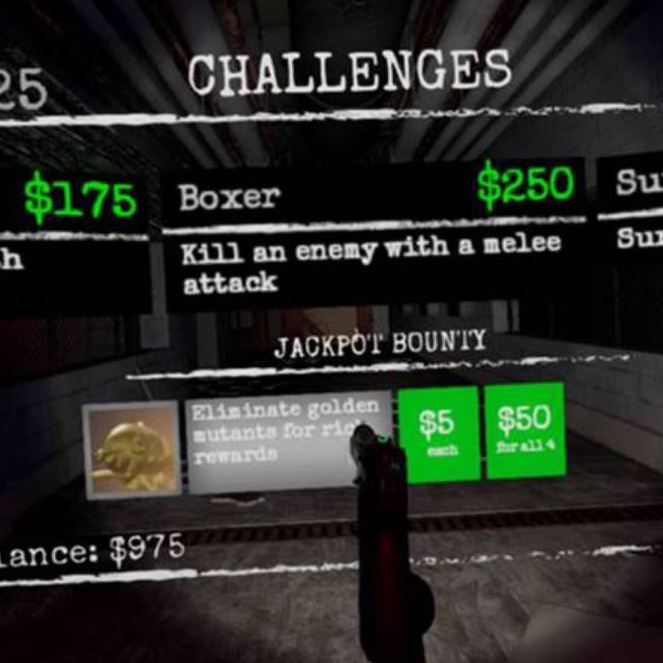
\includegraphics[width=.95\linewidth]{brookhaven.jpg}
  \caption{Brookhaven Experiment (2016)}
\end{subfigure}
\caption{Examples of Virtual Reality Interfaces}
\end{figure*}

\subsection{Usability in Virtual Reality}
The companies and developers at the forefront of the new wave of virtual reality hardware and software have faced many challenges in comfort and usability. Issues with nausea and motion sickness plagued early iterations of head mounted displays. The addition of positional tracking and a greater understanding of significant design choices like locomotion have overcome most of these growing pains.

Now the focus of research is around usability of interfaces in VR. Valve, a driving force in desktop VR, presented some factors of usability at the Game Developer's Conference. When discussing interactions outside the user's area of reach they cited Fitt's law (Malaika 2015). This law has been extended from one dimensional interfaces into 2D interfaces and now into 3D and states that the speed at which a user acquires a target is exponentially proportionate to the size of the target at a given distance (Atsuo 2001). When using a pointer based system, small interface elements at a distance away become very slow to interact with. 

Another notable aspect of ease-of-use regards the placement of interface elements around the user. Due to the 360 degree nature of a 3D interface if the user is constantly required to turn around in order to perform actions it will become fatiguing. Owlchemy labs, developers of Job Simulator and strong proponents of diegetic interfaces build scenarios in such a way that users do not have to turn frequently and generally have direct access to everything they may need at a given time (Schwartz 2015).

\subsection{Testing virtual reality applications}
Testing virtual reality interfaces is something that has little research published about it. There are many articles that cover the preparation and caution required around motion sickness but they glance over the practicalities of collecting data during testing. One transcript of a presentation (Bromley 2016) mentions the issues surrounding communication with a user during tests as they are wearing a headset while participating. One solution the researcher poses is to ask questions between short play sessions. Another is to have a direct line to the player so they can hear you while wearing a headset however this can be distracting and require extra set up for each user. 

The emphasis on avoiding any nauseating situations usually focuses on movement of the user's view outwith their control. As users may be standing during testing it is also advised that the moderator watch them carefully. (Wales 2016)

\section{Methodology}
\subsection{Application}
\subsubsection{Overview and design}
Before being able to apply the two adaptive techniques, dynamic scaling and error analysis, an interface needed to be implemented. The design of the interface and the application as a whole was designed with user testing and data gathering in mind. In order to better understand what the interface would need to provide, several points were devised to outline the core features and constraints:

\begin{itemize}[noitemsep,topsep=0pt]
\item The interface must feature a minimal number of clear interactions for easy learning.
\item The interface must use a laser pointer to interact with elements outwith arms reach.
\item A pressurised environment should be used to encourage users to interact with the interface.
\end{itemize}

Each of these points was taken into consideration and a simple virtual reality application was developed. The interactions considered were those common to many applications but a drag and drop interface was decided upon. This would be intuitive for the users who would only have a few minutes to use the application. Many pieces of existing virtual reality software  show that moving and throwing objects in virtual reality is a gratifying action. Having decided upon the interaction the next step was to select objects to be interacted with.

To maintain the simplicity of the application and to try and avoid users becoming wrapped up in the details of the objects they were interacting with a simple ball was chosen. Initially a more complex object was implemented but as the focus needed to be on interacting and not the objects being interacted with the coloured ball leant itself to the testing. A ball also has associations with grabbing and throwing which reinforced the core interaction.

The choice to use a laser pointer was made early on as there is inherent difficulty in the task of selecting something in 3D space using a pointer. The use of a pressurised environment was executed in the form a timed and scored interface. At first a kind of tutorial in which the user would be prompted to perform different actions was considered. The simple timer system was chosen instead because it did had no reliance on the speed at which the user reads or the interpretation of instructions. By having a single task repeated as many times as possible the user is forced to be less cautious with their interactions, providing more varied data.

The final design of the application took into account the outlined points and consisted of a simple space with a table to focus the user's gaze. On this table balls of two colours appear and roll toward the participant. A timer is visible on the table and is counting down to zero, some text instructs the user to place the balls into a basket of corresponding colour next to the table. Each time the user successfully selects and places a ball a score readout above the basket increases.

\subsubsection{Implementation and Iteration}
The initial design was implemented (as seen in Figure 5) in Unreal Engine 4 using C++ to create the core interaction system and Blueprints (visual scripting) to create the gameplay. By separating the code of the gameplay from that of the interaction it allowed easy iteration and tweaking of the surface features while having a strong, performant foundation in C++. 

Once the implementation was finished an early user test was performed which revealed several issues with the design. Initially two controllers, on in each hand, were used to interact. Both had laser pointers but only one would be used in the dominant hand the other would occasionally obstruct the user's actions. The first implementation also asked the user to place blue balls into one basket and red into another, this meant as the balls appeared the user was constantly interacting and had no time to break.

Although the pressure on the user was intended it quickly became tiring for them to interact and the decision was made to have only one basket so that users would interact with only one colour and need to avoid the other. This would also give more data points for when the user did select a non basket coloured ball the system could tell it was a failed action.

One change made before the final round of user testing expanded upon the interface itself. The applications in a real piece of software for selecting moving objects like the balls rolling toward the user are difficult to imagine. To improve the evaluation and provide a more realistic scenario the interface switches half way through the application's timer from the rolling balls to a grid of static balls suspended away from the user. This also tests the ability to select tightly packed objects something the moving interface of the rolling balls did not do effectively.

\begin{figure*}
\centering
  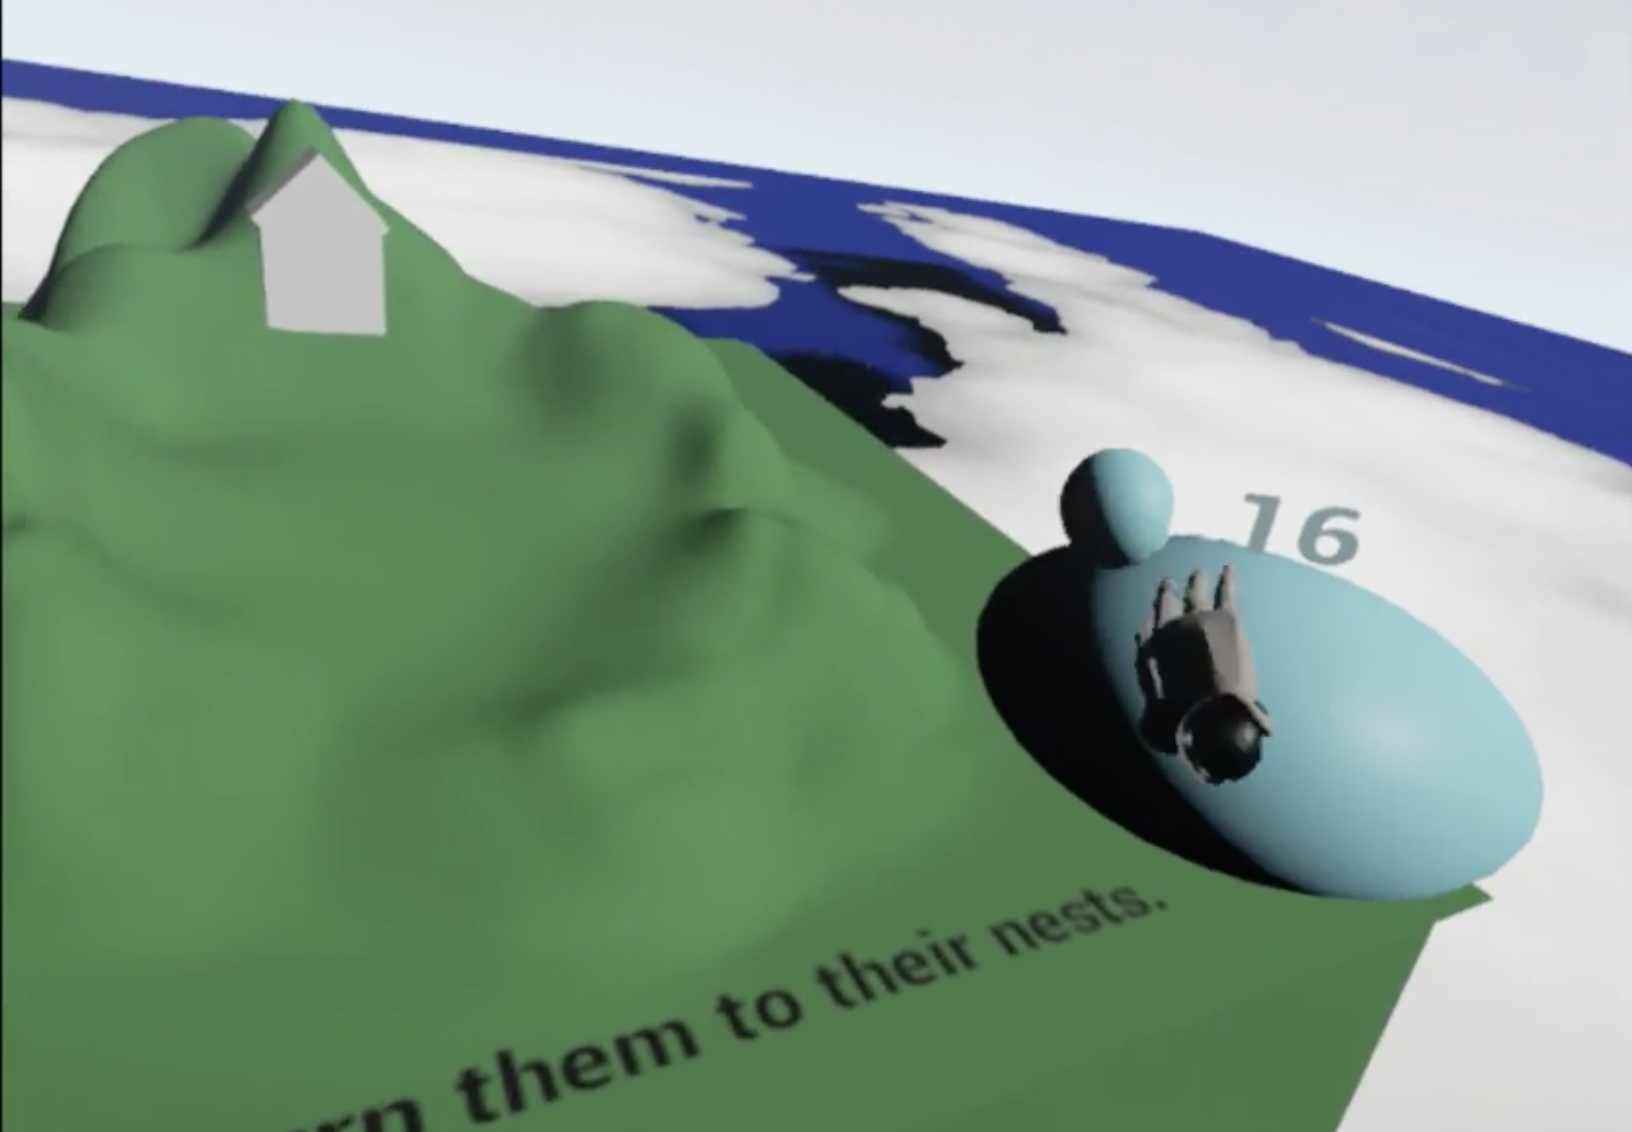
\includegraphics[width=.8\linewidth]{earlydemo.png}
  \caption{Early Iteration}
\end{figure*}


\subsection{Adaptive Techniques}
\subsubsection{Overview}
The research done into adaptive user interfaces and the techniques behind them focused mainly on implementations in 2D scenarios. To apply all of these techniques to 3D would be outside the scope of this project and have made it very difficult to complete the user testing. As such two techniques were chosen and altered for virtual reality. The first is error analysis, with the application requiring only one button for interaction the room for error is small and so easily tracked. The concept of error analysis is to detect when a user has incorrectly pressed a button and somehow react to it.

The second technique chosen was dynamic scaling although in a different form to that found in most of the previous research done on adaptive techniques. Generally the scaling of user interface elements would be done in response to an error, improving a user's ability to select it. By relating the scaling of every element to the predicted selection of the user it can constantly accommodate and assist the interactions with the interface, scaling up areas of focus.

\subsubsection{Error Analysis}
To understand how to know when a user has made an error the underlying interaction system in C++ has to be explained. When designing the interaction system the input is bound to a set of functions. This means that when the user presses the trigger in an attempt to select an element it will run through a series of steps to complete the action:

\begin{itemize}[noitemsep,topsep=0pt]
\item The user presses the trigger.
\item The system runs the grab function.
\item A raycast is sent along the laser pointer.
\item If the raycast intersects any number of elements the first is selected.
\item If the raycast intersects no elements, nothing happens.
\end{itemize}

It can be assumed to a certain probability that if the final step is true and no elements were found, the user made an error. The user could simply have pressed the trigger with no intention to select something but this is something that cannot easily be predicted. But in the case that the user was trying to make a selection and failed error analysis can allow the system to make an educated guess at what the desired element was and take action on it. 

Although this assisted selection would be easily accomplished in 2D by simply choosing the closest element to the cursor, in 3D with a continuous 'beam' cursor going into infinite it is more complex to solve. The implementation uses the shortest distance formula to find which element along the line of the laser pointer is the closest taking the magnitude of the vector forming a right angle to the direction.

\begin{figure*}
\centering
  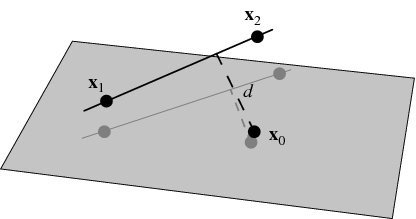
\includegraphics[width=.8\linewidth]{nearestpoint.png}
  \caption{Visualisation of the shortest distance between a vector and a point}
\end{figure*}

By using a threshold distance beyond which elements are ignored the instant the user makes an error the system can search for any that are not overlapping but close enough to select and find the nearest. The basic form of this formula is as follows: 

$d = |(\mathbf{a}-\mathbf{p}) - ((\mathbf{a}-\mathbf{p}) \cdot  \mathbf{n})\mathbf{n}|$

In which $d$ is the shortest distance between point $p$ and the vector with position $a$ and direction $n$. A visualisation of the formula can be seen in figure 6 below. This implementation immediately proved to make selecting moving elements and densely packed elements faster and less cumbersome during basic testing. It could break down when a user is selecting objects very far away through a grouping of close objects in which case the formula could be modified to take into account distance of the perpendicular point along the laser.

\subsubsection{Dynamic Scaling}
The second technique adapts the interface visually in an attempt to improve the usability of smaller or tightly packed elements such as the grid of balls presented in the latter half of the application. By using the shortest distance formula again to determine how far away an element is from the user's laser it can be scaled by some amount to create the effect of it becoming larger as the user goes to select it. The effectiveness of this technique relies on the theory laid out in Fitt's Law stating that the time to select a user interface element is proportionate to its size and the distance from it. By scaling the elements as the distance to it decreases the speed of the selection should increase.

Initially a more complex algorithm was used to scale the elements exponentially and with a slight downsizing at the start. This was intended to make a kind of focus bubble inside which elements would be larger and on the edge of which elements would be smaller. This concept made selection confusing especially when approaching a group of elements from far away as they would all shrink on approach before getting larger at varying rates.

Something that became apparent during the implementation of the adaptive scaling was the importance of consistency. Early testing made it seem that if the user expects something to happen to the interface dynamically that becomes something they will compensate for in the interaction with the interface. As soon as something breaks the consensus it is no longer reliable and could hinder usability.

The scaling of the object was applied to the mesh itself but not the collider, this would cause issues where the mesh would begin clipping into nearby static, unelectable meshes and would sometimes seem like a property of the element and not the interface in general. By simply adding a kind of highlight replica of the mesh with transparency and scaling this instead, each element could be seen at its native scale at all times yet the dynamic scaling could still be applied. This highlight mesh was also used for the static interface to show when an object was in range to be selected by becoming visible.

\subsubsection{Further considerations}
When implementing these adaptive techniques there were several other approaches considered. Stabilisation of the laser pointer could be used to snap to nearby elements like a pre-emptive error analysis so that if the user would have slightly missed an element the system snaps the laser to it before they even select it. This was not used as the constant change of direction and lack of fine control over the laser could be disorientating and nauseating.

Another way to adapt the interface would be by modelling the user and adjusting the environment to them, this could be done in a number of ways. For example taking the user's height and scaling the entire interface to be proportionate to them. As the focus of the research and implementation was on an experience that could be accessed and used in only a few minutes the calibration required for this technique went against the project design.

Other than the input of the laser pointer and the button for selection the direction the user is facing could perhaps be used to improve the error analysis. This approach would take not only the closest element to the laser into account but also the closest element to the gaze of the user. As the user testing would already require the control test alongside the two techniques adding a third test for this iteration on error analysis did not seem beneficial.

\subsection{Evaluation}
\subsubsection{Overview}
To evaluate the effectiveness of the two adaptive interface techniques a single virtual reality interface was constructed as described in 4.1.2, the basic version of this was used as the static control. Alongside this interface, which users would interact with for a minute under a timer, the same interface but with the adaptive techniques applied individually. This would give the data to compare and evaluate their impact on usability.

\subsubsection{Data Gathering}
By gathering data from the application in the background the performance of the user could be analysed and compared for the static control and each technique. Alongside the questionnaire data this would give a solid understanding of how the user perceived the usability and how their interaction with the interface was actually affected.

The data gathering system was a simple messaging model that wrote out an xml formatted file which could then be read back into the Unreal Engine Editor and played back in 3D akin to a video capture. This proved to be useful when looking for errors in the development as well as for analysing a user's performance.

A single object, the data gatherer, writes to a file at a specified tick while the application is running. Every tick it stores the name, position and rotation of every object it is currently tracking. In order for an object to be tracked it must have a specific data generator component used to communicate with the data gatherer. When initialising this component the data gatherer adds the object's name to its list to keep track of it. The name can then be used to request the required information.

Although this data alone is enough to reconstruct a user's interactions with the interface visually it does not keep track of the results of their interactions. To do this a second event layer was added the communication between data generator components and the data gatherer. When the component creates an event the data gatherer stores it at the tick during which it occurred along with the name of the object that generated it and some description. This allows every error, success and other non-visual interactions to be store and replayed easily.

At first the data gathering system would output large amounts of data every frame causing performance loss and discomfort when using the application. To account for this a simple distance threshold was added so that each tracked object's information is only updated when it has moved a certain amount. When replaying data in the editor a simple interpolation can smooth out this loss of data.

\subsubsection{Questionnaire}
To allow the users to feedback on the application and provide a counterpoint to the data gathered by the application which may not fully represent the user experience, a series of questions was devised and given to the user between the testing of each technique and the control (See Appendix A). The questions aimed to provide a variety of both negative and positive feedback while being vague enough to allow users to focus on the experience and not be caught up in their interpretation of each question.

The final form of the questions is an iteration on the System Usability Scale which is widely used as a tool for measuring usability of a system. The decision to use the term system instead of interface would allow the user to consider not just the physical interface but the interaction with the interface as well. The scale uses a five option system ranging from 'strongly agree' to 'strongly disagree'. This range gives enough room for comparison without overwhelming the tester with choices. 

As in the standard Scale 10 questions were asked although slightly adapted from the ones given. The main addition was the final question regarding comfort. A vital component of usability in virtual reality specifically is user comfort. As there is a tendency for user's to associate their comfort with the experience itself by using this question to weigh the answers of the testers any especially bad experiences and the answers associated could be offset.

When user testing the order of the tests for the static control interface and two adaptive techniques was randomised. The user would enter the room, be briefed and then asked to complete the consent form. Once they were ready they were placed in the headset and left to interact with the minute long timed interface. When the timer expired the headset was removed and they completed the questionnaire. This was repeated until each iteration of the interface had been tested in a random order. To ensure that each user tested each interface in each order a balanced number of times a simple list of the interface iteration to be tested was devised and followed rather than letting the system randomise the techniques applied.

\section{Results and Discussion}
\subsection{Qualitative Data}
\subsubsection{Overview of Results}
The data from the ten questionnaire responses gathered throughout the testing process were collected in a spreadsheet and analysed by assigning a value of 1 - strongly disagree to 5 - strongly agree to each answer. Certain answers were weighted negatively based on the phrasing of the question i.e. "7. I found the system very cumbersome to use.", others were weighted positively i.e. "3. I thought the system was easy to use.". Each questionnaire is split into three sections A, B and C, corresponding to the iterations of the interface tested by each user. 

Each section consisted of the same ten questions (see Appendix A). Section A corresponds to the 'static' interface which does not implement any adaptive techniques. Section B corresponds to the 'error analysis' interface which adapts based on user error. Section C corresponds to the 'dynamic scaling' interface which adapts the size of each element as the user approaches them. These questions focus on the user's experience interacting with the system, by averaging the responses received over the ten tests and comparing each section's results it gives an idea of which interface iteration users collectively preferred.

Although the users were not asked to directly compare the experience of the different iterations it can be assumed, to some degree, that their responses are scaled based on their impression of the previous interface. Also note that users were given the three interface iterations in a shuffled order without knowing which was the control. This means a user who experienced the 'static' control interface first may have responded to the adaptive iterations differently to a user experiencing the adaptive iterations before the control.

\subsubsection{Breakdown of responses}
Table 1 shows the average of each response taken for the ten responses across all three sections of the questionnaire. As explained in 5.1.1 certain questions are weighted negatively based on the phrasing given. These are questions 2, 5, 7 and 9 all proceeded by a minus sign in Table 1. In order to visualise the data in a more understandable and comparable way the negatively weighted answers were translated onto a reverse scale with 1 being strongly agree and 5 being strongly disagree. This means an answer to a negative question of agree - 4 on the normal scale becomes disagree - 2 on the reverse scale essentially taking the positive version of it. These translated negative answers alongside the other positive answers were then compiled into graphs as shown in Figure 7. Both the line graph and bar chart use the same data and provide some insight into the user experience for each iteration of the interface.

Looking at the line graph it is clear that the responses to Section B, the error-based adaptive technique, are the most positive in almost every question. Section A, the static control interface, is the most negative in almost every question. Finally Section C, the dynamic scaling technique, is the midground in almost every question. The primary exceptions to these outcomes are question 5 and  question 9. Question 5: "I thought there was too much inconsistency in this system.", received slightly more positive answers in Section C than Section B. This could be that although the adaptive error-analysis was perceived as easier to use when it failed to act as the user expected it caused more issues than the dynamic scaling. Question 9 on the other hand: "I needed to learn a lot of things before I could get going with this system." received more positive answers in Section A, the static control interface by a small margin. This could be attributed to the need to grasp what how the interface is adapting when the dynamic scaling and error-analysis adaptive techniques are applied. Even though they may make the interface easier to use, they create slightly more of a learning curve than a static interface.

\begin{table}
\centering
\begin{tabular}{ |c|c|c|c|c|c|c|c|c|c|c|c| } 
 \hline
 \textbf{Question} & \textbf{1} & \textbf{2} & \textbf{3} & \textbf{4} & \textbf{5} & \textbf{6} & \textbf{7} & \textbf{8} & \textbf{9} & \textbf{10} & \textbf{Total} \\ 
 \hline
 \textbf{Section A} & 3.2 & -1.7 & 3.7 & 3.7 & -2.7 & 4.0 & -2.7 & 3.5 & -1.4 & 3.8 & 13.4\\ 
 
 \textbf{Section B} & 3.9 & -1.3 & 4.1 & 4.4 & -1.7 & 4.5 & -2.4 & 3.9 & -1.6 & 4.3 & 18.1\\ 
 
 \textbf{Section C} & 3.8 & -1.8 & 3.9 & 4.0 & -1.5 & 4.3 & -2.3 & 3.9 & -1.7 & 4.1 & 16.7\\ 
 \hline
\end{tabular}
\caption{Averaged responses over ten users}
\end{table}

\begin{figure}
\begin{subfigure}{.5\textwidth}
\centering
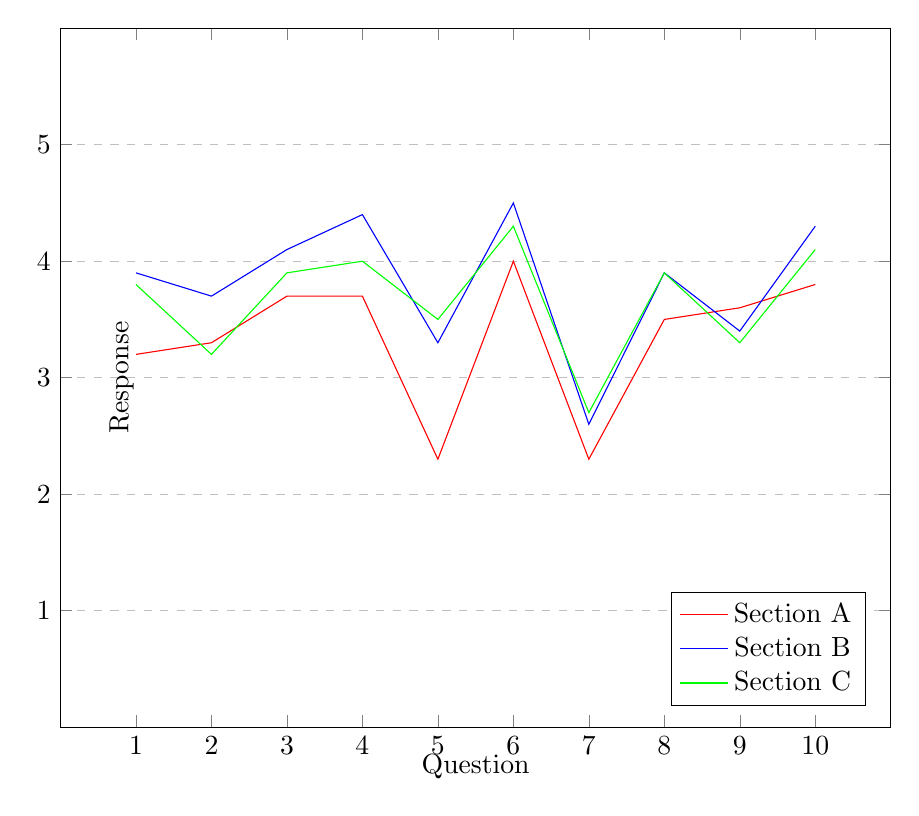
\begin{tikzpicture}
\begin{axis}[
    xlabel={Question},
    ylabel={Response},
    x label style={at={(axis description cs:0.5,-0.025)},anchor=north},
    y label style={at={(axis description cs:0.1,.5)},anchor=south},
    xmin=0, xmax=11,
    ymin=0, ymax=6,
    xtick={1,2,3,4,5,6,7,8,9,10},
    ytick={1,2,3,4,5},
    legend pos=south east,
    ymajorgrids=true,
    grid style=dashed,
 	width=1\textwidth,
]
 
\addplot[
    color=red,
    mark=circle,
    ]
    coordinates {
    (1,3.2)(2,3.3)(3,3.7)(4,3.7)(5,2.3)(6,4.0)(7,2.3)(8,3.5)(9,3.6)(10,3.8)
    };
 
\addplot[
    color=blue,
    mark=circle,
    ]
    coordinates {
    (1,3.9)(2,3.7)(3,4.1)(4,4.4)(5,3.3)(6,4.5)(7,2.6)(8,3.9)(9,3.4)(10,4.3)
    };
    
\addplot[
    color=green,
    mark=circle,
    ]
    coordinates {
    (1,3.8)(2,3.2)(3,3.9)(4,4.0)(5,3.5)(6,4.3)(7,2.7)(8,3.9)(9,3.3)(10,4.1)
    };
    \legend{Section A, Section B, Section C}
    
\end{axis}
\end{tikzpicture}
\caption{Graph of averaged responses}
\end{subfigure}%
\begin{subfigure}{.5\textwidth}
\centering
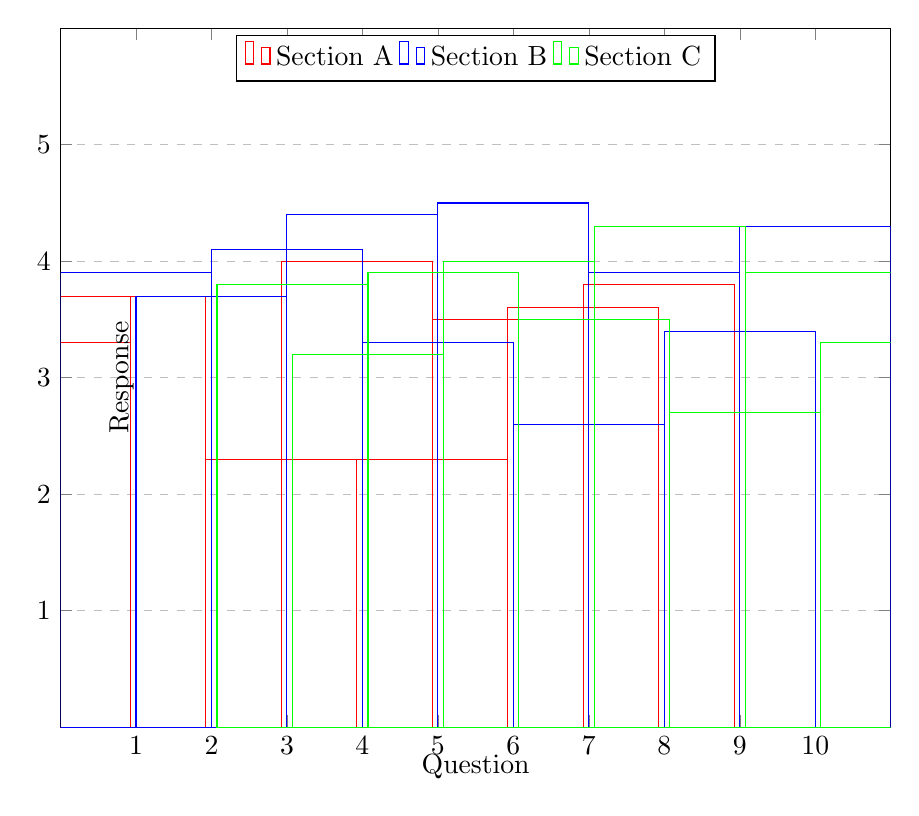
\begin{tikzpicture}
\begin{axis}[
 	ylabel=Response,
 	xlabel=Question,
    x label style={at={(axis description cs:0.5,-0.025)},anchor=north},
    y label style={at={(axis description cs:0.1,.5)},anchor=south},
    xmin=0, xmax=11,
    ymin=0, ymax=6,
    xtick={1,2,3,4,5,6,7,8,9,10},
    ytick={1,2,3,4,5},
 	legend style={at={(0.5,0.99)},
 	anchor=north,legend columns=-1},
 	ybar,
 	bar width = 2,
    ymajorgrids=true,
    grid style=dashed,
    xtick align=inside,
 	width=1\textwidth,
 	]
 
\addplot[
    color=red,
    ]
    coordinates {
    (1,3.2)(2,3.3)(3,3.7)(4,3.7)(5,2.3)(6,4.0)(7,2.3)(8,3.5)(9,3.6)(10,3.8)
    };
 
\addplot[
    color=blue,
    ]
    coordinates {
    (1,3.9)(2,3.7)(3,4.1)(4,4.4)(5,3.3)(6,4.5)(7,2.6)(8,3.9)(9,3.4)(10,4.3)
    };
    
\addplot[
    color=green,
    ]
    coordinates {
    (1,3.8)(2,3.2)(3,3.9)(4,4.0)(5,3.5)(6,4.3)(7,2.7)(8,3.9)(9,3.3)(10,4.1)
    };
    \legend{Section A, Section B, Section C}
    
\end{axis}
\end{tikzpicture}
\caption{Chart of averaged responses}
\end{subfigure}

\caption{Visualisation of response data}
\end{figure}

\subsubsection{Analysis}
Taking the data and its representations into account it is clear that users found the adaptive techniques to be beneficial to the user experience and usability of the interfaces. The static interface is consistently deemed harder to use, more cumbersome and users felt less confident when using it. In comparison the two adaptive techniques were very closely regarded by users and only by a tiny fraction was the error-analysis interface (Section B) more positively received. This is considering that the results shown are averages of all ten responses. In some individual cases the adaptive techniques equally usable but very rarely less usable than the static control. The full results are in Appendix B.

Something to note about the two exceptions mentioned in 5.1.2, Question 5 and Question 9, is that they were two of the four negatively weighted questions along with 2 and 7. This could also have affected the responses given as there was a tendency to give answers that always provided positive feedback. On average no user gave an answer of 'disagree' or 'strongly disagree' to the positively weighted answers or 'agree'/'strongly agree' to the negatively weighted answers. This shows that the interfaces in general were found to be usable despite the static interface being less well received than the adaptive interfaces.

\subsection{Quantitative Data}
\subsubsection{Overview of Results}
During user testing all sessions were recorded using the data gathering system described in 4.3.2. The output data for each user session was categorised by the section being tested i.e. A, B or C. By using a simple python script to analyse these output .xml files some useful data points were extracted. The application focuses on the single user interaction of grabbing and so to measure the effectiveness and usability of an interface the ability of the user to grab the elements should correspond to their ability to use the interface as a whole. Every time a user attempts to grab an object an event is sent to the data gatherer and output along with whether the grab was successful and if the object grabbed is correct. To analyse the data, the number of occurrences of each of these three 'grab types' was counted and gathered into a table (see Appendix C). 

The count of how many times a user has performed a 'successful', 'failed' or 'incorrect' grab varies greatly between users as they each interact at different rates and with different outcomes. However by averaging the counts across all participants an idea of the overall ratio between the grab types was attained as seen in Table 2 and Figure 8. Each iteration of the interface tested by the users was split into two 'phases' as explained in 4.1.2. Phase 1 has the user grab rolling balls and place them in the basket whereas Phase 2 has users grab the balls from a large static grid in front of them. In Figure 8 the line on each bar represents the point during testing when the interface switched from Phase 1 to Phase 2. For example in Section A the average number of total successful grabs was around 30 but only 10 of those occurred during Phase 1.

\begin{table}
\centering
\vspace{1cm}\begin{tabular}{ |c|c|c|c|c|c|c|c|c|c| }
 	\hline
 	\textbf{Phase} & \multicolumn{3}{|c|}{\textbf{Phase 1 and 2}} &  \multicolumn{3}{|c|}{\textbf{Phase 1}} & \multicolumn{3}{|c|}{\textbf{Phase 2}} \\
 	\hline
	\textbf{Section} & \textbf{A} & \textbf{B} & \textbf{C} & \textbf{A} & \textbf{B} & \textbf{C} & \textbf{A} & \textbf{B} & \textbf{C} \\
	\hline
	\textbf{Successful Grabs} & 29.9 & 45.5 & 34.1 & 18.8 & 26.5 & 23.5 & 11.1 & 19 & 10.6 \\
	\hline
	\textbf{Failed Grabs} & 22 & 1.9 & 16.3 & 9.2 & 0.1 & 7.2 & 12.8 & 1.8 & 9.1 \\
	\hline
	\textbf{Incorrect Grabs} & 24.5 & 37 & 28.5 & 18.8 & 26.4 & 23.2 & 5.7 & 10.6 & 5.3 \\
	\hline
\end{tabular}
\caption{Average grab counts for Phase 1 and 2}
\end{table}


\begin{figure}
\centering 
\hspace{-1cm}\begin{tikzpicture}
\begin{axis}[
 	ylabel=Count,
 	xlabel=Grab Type,
    x label style={at={(axis description cs:0.5,-0.05)},anchor=north},
 	ymin = 0,
 	symbolic x coords={Successful,Failed,Incorrect},
    xtick=data,
 	ybar,
 	enlarge x limits=0.2,
 	bar width = 20pt,
 	width=0.7\textwidth,
]
 
\addplot[
    color=red,
    ]
    coordinates {
    (Successful,29.9)(Failed,22)(Incorrect,24.5)
    };
 
\addplot[
    color=blue,
    ]
    coordinates {
    (Successful,45.5)(Failed,1.9)(Incorrect,37)
    };
    
\addplot[
    color=green,
    ]
    coordinates {
    (Successful,34.1)(Failed,16.3)(Incorrect,28.5)
    };
   
\draw[red, very thick] (-31,111) -- (-12,111);
\draw[blue, very thick] (-10,190) -- (10,190);
\draw[green, very thick] (12,106) -- (31,106);

\draw[red, very thick] (69,128) -- (88,128);
\draw[blue, very thick] (90,18) -- (110,18);
\draw[green, very thick] (112,91) -- (132,91);

\draw[red, very thick] (168,57) -- (188,57);
\draw[blue, very thick] (190,106) -- (210,106);
\draw[green, very thick] (212,53) -- (232,53);
    
    \legend{Section A, Section B, Section C}    
\end{axis}
\end{tikzpicture}
\caption{Chart of average grab counts}
\end{figure}


\subsubsection{Breakdown of data points}


\subsubsection{Final analysis}

\subsection{Comparison}
\subsubsection{Overview of Results}

\subsubsection{Qualitative vs quantitative}

\section{Conclusion}

\pagebreak

\section{Appendices}

\subsection{Appendix A}

\begin{enumerate}
\item I think that I would like to use this system frequently.
\item I found the system unnecessarily complex. 
\item I thought the system was easy to use. 
\item I found the various functions in this system were well integrated. 
\item I thought there was too much inconsistency in this system. 
\item I would imagine that most people would learn to use this system very quickly. 
\item I found the system very cumbersome to use. 
\item I felt very confident using the system.
\item I needed to learn a lot of things before I could get going with this system. 
\item I felt comfortable while using this system.
\end{enumerate}

\vspace*{-1.25cm}\subsection{Appendix B}

\begin{table}[!ht]
\centering
\hspace*{-2.5cm}\begin{tabular}{ |l|l|l|l|l|l|l|l|l|l|l|l|l|l|l|l|l|l|l|l|l|l|l|l|l|l|l|l|l|l|l| }
 	\hline
	\multirow{2}{*}{\textbf{User}} & \multicolumn{10}{|c|}{\textbf{Section A (Questions)}} & \multicolumn{10}{|c|}{\textbf{Section B (Questions)}} & \multicolumn{10}{|c|}{\textbf{Section C (Questions)}} \\
	 & \textbf{1} & \textbf{2} & \textbf{3} & \textbf{4} & \textbf{5} & \textbf{6} & \textbf{7} & \textbf{8} & \textbf{9} & \textbf{10} & \textbf{1} & \textbf{2} & \textbf{3} & \textbf{4} & \textbf{5} & \textbf{6} & \textbf{7} & \textbf{8} & \textbf{9} & \textbf{10} & \textbf{1} & \textbf{2} & \textbf{3} & \textbf{4} & \textbf{5} & \textbf{6} & \textbf{7} & \textbf{8} & \textbf{9} & \textbf{10} \\
	\hline
	\textbf{1} & 4 & 1 & 5 & 5 & 2 & 5 & 1 & 5 & 1 & 5 & 5 & 1 & 5 & 5 & 1 & 5 & 1 & 5 & 1 & 5 & 5 & 1 & 5 & 5 & 1 & 5 & 1 & 5 & 1 & 5 \\
	\hline
	\textbf{2} & 2 & 2 & 2 & 1 & 5 & 4 & 2 & 1 & 1 & 3 & 3 & 1 & 4 & 4 & 2 & 5 & 1 & 3 & 1 & 4 & 3 & 1 & 3 & 3 & 4 & 5 & 2 & 3 & 1 & 4 \\
	\hline
	\textbf{3} & 5 & 1 & 5 & 5 & 2 & 5 & 2 & 5 & 1 & 5 & 3 & 1 & 3 & 4 & 1 & 3 & 4 & 2 & 2 & 3 & 4 & 1 & 4 & 5 & 1 & 4 & 3 & 3 & 2 & 4 \\
	\hline
	\textbf{4} & 3 & 1 & 2 & 3 & 4 & 3 & 4 & 3 & 1 & 3 & 4 & 1 & 4 & 5 & 1 & 5 & 2 & 5 & 1 & 5 & 4 & 2 & 3 & 4 & 1 & 5 & 3 & 5 & 1 & 4 \\
	\hline
	\textbf{5} & 3 & 2 & 5 & 5 & 1 & 4 & 3 & 4 & 1 & 4 & 5 & 1 & 5 & 5 & 4 & 5 & 4 & 4 & 1 & 5 & 5 & 1 & 5 & 4 & 1 & 5 & 1 & 5 & 1 & 5 \\
	\hline
	\textbf{6} & 4 & 1 & 4 & 4 & 2 & 5 & 2 & 4 & 1 & 5 & 5 & 1 & 5 & 5 & 1 & 5 & 1 & 5 & 1 & 5 & 5 & 1 & 5 & 5 & 1 & 5 & 1 & 5 & 1 & 5 \\
	\hline
	\textbf{7} & 3 & 2 & 4 & 3 & 3 & 4 & 4 & 3 & 1 & 4 & 4 & 2 & 4 & 4 & 1 & 5 & 2 & 4 & 3 & 4 & 4 & 1 & 4 & 4 & 1 & 5 & 2 & 4 & 2 & 4 \\
	\hline
	\textbf{8} & 2 & 3 & 3 & 2 & 5 & 1 & 4 & 2 & 4 & 2 & 4 & 2 & 3 & 3 & 3 & 3 & 4 & 2 & 3 & 3 & 2 & 4 & 2 & 2 & 3 & 2 & 4 & 2 & 3 & 2 \\
	\hline
	\textbf{9} & 4 & 1 & 4 & 5 & 1 & 5 & 2 & 5 & 1 & 4 & 3 & 1 & 4 & 5 & 1 & 5 & 3 & 5 & 1 & 5 & 3 & 2 & 5 & 4 & 1 & 5 & 4 & 4 & 1 & 5 \\
	\hline
	\textbf{10} & 2 & 3 & 3 & 4 & 2 & 4 & 3 & 3 & 2 & 3 & 3 & 2 & 4 & 4 & 2 & 4 & 2 & 4 & 2 & 4 & 3 & 4 & 3 & 4 & 1 & 2 & 2 & 3 & 4 & 3 \\
	\hline
\end{tabular}
\caption{Full results from questionnaire}
\end{table}

\subsection{Appendix C}

\begin{table}[!ht]
\centering
\begin{tabular}{ |c|c|c|c|c|c|c|c|c|c|c|c|c|c|c|c| }
 	\hline
	\textbf{Participant} & \multicolumn{3}{|c|}{\textbf{1}} &  \multicolumn{3}{|c|}{\textbf{2}} & \multicolumn{3}{|c|}{\textbf{3}} & \multicolumn{3}{|c|}{\textbf{4}} & \multicolumn{3}{|c|}{\textbf{5}} \\
	\hline
	\textbf{Section} & \textbf{A} & \textbf{B} & \textbf{C} & \textbf{A} & \textbf{B} & \textbf{C} & \textbf{A} & \textbf{B} & \textbf{C} & \textbf{A} & \textbf{B} & \textbf{C} & \textbf{A} & \textbf{B} & \textbf{C} \\
	\hline
	\textbf{Successful Grabs} & 27 & 47 & 35 & 34 & 40 & 45 & 32 & 45 & 32 & 20 & 39 & 17 & 38 & 61 & 36 \\
	\hline
	\textbf{Failed Grabs} & 13 & 0 & 8 & 18 & 2 & 21 & 17 & 0 & 18 & 20 & 1 & 13 & 45 & 6 & 32 \\
	\hline
	\textbf{Incorrect Grabs} & 24 & 38 & 28 & 28 & 33 & 40 & 25 & 32 & 24 & 19 & 31 & 14 & 29 & 49 & 30 \\
	\hline
\end{tabular}

\centering
\vspace{1cm}\begin{tabular}{ |c|c|c|c|c|c|c|c|c|c|c|c|c|c|c|c| }
 	\hline
	\textbf{Participant} & \multicolumn{3}{|c|}{\textbf{6}} & \multicolumn{3}{|c|}{\textbf{7}} & \multicolumn{3}{|c|}{\textbf{8}} & \multicolumn{3}{|c|}{\textbf{9}} & \multicolumn{3}{|c|}{\textbf{10}} \\
	\hline
	\textbf{Section} & \textbf{A} & \textbf{B} & \textbf{C} & \textbf{A} & \textbf{B} & \textbf{C} & \textbf{A} & \textbf{B} & \textbf{C} & \textbf{A} & \textbf{B} & \textbf{C} & \textbf{A} & \textbf{B} & \textbf{C} \\
	\hline
	\textbf{Successful Grabs} & 17 & 39 & 35 & 27 & 51 & 34 & 38 & 46 & 39 & 32 & 39 & 34 & 34 & 48 & 34 \\
	\hline
	\textbf{Failed Grabs} & 18 & 3 & 10 & 36 & 1 & 18 & 27 & 4 & 16 & 16 & 2 & 18 & 10 & 0 & 9 \\
	\hline
	\textbf{Incorrect Grabs} & 13 & 29 & 30 & 21 & 46 & 30 & 32 & 39 & 32 & 25 & 30 & 28 & 29 & 43 & 29 \\
	\hline
\end{tabular}

\caption{Full results from data gathered}
\end{table}


\begin{table}[!ht]
\centering
\begin{tabular}{ |c|c|c|c|c|c|c|c|c|c|c|c|c|c|c|c| }
 	\hline
	\textbf{Participant} & \multicolumn{3}{|c|}{\textbf{1}} &  \multicolumn{3}{|c|}{\textbf{2}} & \multicolumn{3}{|c|}{\textbf{3}} & \multicolumn{3}{|c|}{\textbf{4}} & \multicolumn{3}{|c|}{\textbf{5}} \\
	\hline
	\textbf{Section} & \textbf{A} & \textbf{B} & \textbf{C} & \textbf{A} & \textbf{B} & \textbf{C} & \textbf{A} & \textbf{B} & \textbf{C} & \textbf{A} & \textbf{B} & \textbf{C} & \textbf{A} & \textbf{B} & \textbf{C} \\
	\hline
	\textbf{Successful Grabs} & 10 & 18 & 12 & 13 & 14 & 13 & 13 & 24 & 14 & 2 & 17 & 4 & 17 & 29 & 14 \\
	\hline
	\textbf{Failed Grabs} & 6 & 0 & 3 & 7 & 2 & 13 & 14 & 0 & 14 & 11 & 1 & 8 & 30 & 6 & 21 \\
	\hline
	\textbf{Incorrect Grabs} & 7 & 10 & 5 & 7 & 7 & 9 & 6 & 11 & 6 & 1 & 9 & 1 & 8 & 17 & 9 \\
	\hline
\end{tabular}

\centering
\vspace{1cm}\begin{tabular}{ |c|c|c|c|c|c|c|c|c|c|c|c|c|c|c|c| }
 	\hline
	\textbf{Participant} & \multicolumn{3}{|c|}{\textbf{6}} & \multicolumn{3}{|c|}{\textbf{7}} & \multicolumn{3}{|c|}{\textbf{8}} & \multicolumn{3}{|c|}{\textbf{9}} & \multicolumn{3}{|c|}{\textbf{10}} \\
	\hline
	\textbf{Section} & \textbf{A} & \textbf{B} & \textbf{C} & \textbf{A} & \textbf{B} & \textbf{C} & \textbf{A} & \textbf{B} & \textbf{C} & \textbf{A} & \textbf{B} & \textbf{C} & \textbf{A} & \textbf{B} & \textbf{C} \\
	\hline
	\textbf{Successful Grabs} & 8 & 14 & 9 & 8 & 16 & 9 & 13 & 22 & 12 & 13 & 19 & 10 & 14 & 17 & 9 \\
	\hline
	\textbf{Failed Grabs} & 9 & 2 & 3 & 22 & 1 & 10 & 15 & 4 & 8 & 9 & 2 & 8 & 5 & 0 & 3 \\
	\hline
	\textbf{Incorrect Grabs} & 4 & 4 & 4 & 2 & 11 & 5 & 7 & 15 & 6 & 6 & 10 & 4 & 9 & 12 & 4 \\
	\hline
\end{tabular}

\caption{Phase 1 results from data gathered}
\end{table}

\begin{table}[!ht]
\centering
\begin{tabular}{ |c|c|c|c|c|c|c|c|c|c|c|c|c|c|c|c| }
 	\hline
	\textbf{Participant} & \multicolumn{3}{|c|}{\textbf{1}} &  \multicolumn{3}{|c|}{\textbf{2}} & \multicolumn{3}{|c|}{\textbf{3}} & \multicolumn{3}{|c|}{\textbf{4}} & \multicolumn{3}{|c|}{\textbf{5}} \\
	\hline
	\textbf{Section} & \textbf{A} & \textbf{B} & \textbf{C} & \textbf{A} & \textbf{B} & \textbf{C} & \textbf{A} & \textbf{B} & \textbf{C} & \textbf{A} & \textbf{B} & \textbf{C} & \textbf{A} & \textbf{B} & \textbf{C} \\
	\hline
	\textbf{Successful Grabs} & 17 & 29 & 23 & 21 & 26 & 32 & 19 & 21 & 18 & 18 & 22 & 13 & 21 & 32 & 22 \\
	\hline
	\textbf{Failed Grabs} & 7 & 0 & 5 & 11 & 0 & 8 & 3 & 0 & 4 & 9 & 0 & 5 & 15 & 0 & 11 \\
	\hline
	\textbf{Incorrect Grabs} & 17 & 28 & 23 & 21 & 26 & 31 & 19 & 21 & 18 & 18 & 22 & 13 & 21 & 32 & 21 \\
	\hline
\end{tabular}

\centering
\vspace{1cm}\begin{tabular}{ |c|c|c|c|c|c|c|c|c|c|c|c|c|c|c|c| }
 	\hline
	\textbf{Participant} & \multicolumn{3}{|c|}{\textbf{6}} & \multicolumn{3}{|c|}{\textbf{7}} & \multicolumn{3}{|c|}{\textbf{8}} & \multicolumn{3}{|c|}{\textbf{9}} & \multicolumn{3}{|c|}{\textbf{10}} \\
	\hline
	\textbf{Section} & \textbf{A} & \textbf{B} & \textbf{C} & \textbf{A} & \textbf{B} & \textbf{C} & \textbf{A} & \textbf{B} & \textbf{C} & \textbf{A} & \textbf{B} & \textbf{C} & \textbf{A} & \textbf{B} & \textbf{C} \\
	\hline
	\textbf{Successful Grabs} & 9 & 25 & 26 & 19 & 35 & 25 & 25 & 24 & 27 & 19 & 20 & 24 & 20 & 31 & 25 \\
	\hline
	\textbf{Failed Grabs} & 9 & 1 & 7 & 14 & 0 & 8 & 12 & 0 & 8 & 7 & 0 & 10 & 5 & 0 & 6 \\
	\hline
	\textbf{Incorrect Grabs} & 9 & 25 & 26 & 19 & 35 & 25 & 25 & 24 & 26 & 19 & 20 & 24 & 20 & 31 & 25 \\
	\hline
\end{tabular}

\caption{Phase 2 results from data gathered}
\end{table}

\pagebreak

\section{References}
Anastasios, K. 2012. \emph{When You Shouldn't Use Fitts's Law To Measure User Experience} Smashing. 

Atsuo, M. 2001. \emph{Extending Fitts' law to a three-dimensional pointing task} Japan. Elsevier. 

Bromley, S. 2016. \emph{Running User Tests for Virtual Reality} User Research. Available at: \url{http://www.stevebromley.com/blog/2016/06/03/running-user-tests-for-virtual-reality/} [Accessed March 2017]

Brusilovsky, P. 2000. \emph{Adaptive Hypermedia and Adaptive Web-Based Systems} Italy. Springer.

Bye, K. 2016. \emph{Five Universal Tasks of 3D User Interfaces with Doug Bowman} Voices of VR. Available at: \url{http://voicesofvr.com/five-universal-tasks-of-3d-user-interfaces-with-doug-bowman/} [Accessed November 2016]

Jen, H. 2016. \emph{Designing for VR: Applying Usability Heuristics to Virtual Reality} Omobono. 

Jeremy, L. 2014. \emph{A survey of plasticity in 3D user interfaces} Minneapolis. IEEE. 

Karthik, R. 2011. \emph{Modeling error-based Adaptive User Interfaces} Iowa State University. 

Malaika, Y. 2015. \emph{Interaction Design in VR: Valve's Lessons } Available from: \url{https://www.youtube.com/watch?v=_vQo0ApkAtI} [Accessed October 2016]

Merki, R. 2016. \emph{How VR Analytics Makes Your Product Better} Available from: \url{http://cognitivevr.co/blog/how-vr-analytics-makes-your-product-better/} [Accessed October 2016]

Meyer, R. 2015 \emph{Even Early Focus Groups Hated Clippy} Available from: \url{http://www.theatlantic.com/technology/archive/2015/06/clippy-the-microsoft-office-assistant-is-the-patriarchys-fault/396653/} [Accessed October 2016]

Morgan, K. 1998. \emph{Intelligent User Interfaces: An Introduction} San Fransisco. RUIU 

Northway, C. 2016. \emph{Menus Suck} VRDC. Available at: \url{http://www.gdcvault.com/play/1023668/Menus} [Accessed November 2016]

Pino, N. 2016 \emph{HTC Vive review} Available at: \url{http://www.techradar.com/reviews/wearables/htc-vive-1286775/review/3} [Accessed October 2016]

Robert, Z. \emph{Look-That-There: Exploiting Gaze in Virtual Reality Interactions} Providence. Brown University. 

Schwartz, A. 2015. \emph{Being There: Designing Standing VR Experiences with Tracked Controllers} Available from: \url{https://www.youtube.com/watch?v=hjc7AJwZ4DI} [Accessed October 2016]

Seeto, D. 2016 \emph{Gamestop: PSVR Exceeding Expectations As More Units Are Received For Holiday Season} Online. \url{http://attackofthefanboy.com/news/gamestop-playstation-vr-exceeding-expectations-units-received-holiday-season/} [Accessed October 2016]

\emph{Tilt Brush.} 2016. [software]. HTC Vive. Google. 

\emph{Unreal Engine 4.} 2012. [software]. Windows. Epic Games. 

Wales, J. 2016 \emph{The reality of virtual reality testing} Bunnyfoot. Available at: \url{http://www.bunnyfoot.com/blog/2016/07/the-reality-of-virtual-reality-user-testing-our-top-tips/} [Accessed March 2017]


\section{Bibliography}
Alger, M. 2015. \emph{VR Interface Design Manifesto} Available from: \url{https://www.youtube.com/watch?v=n3b8hZ5NV2E} [Accessed October 2016]

Casey, H. 2015. \emph{Designing For Virtual Reality} Online. UsTwo. [Accessed October 2016]

Julie, J. 2011. \emph{Human-Computer Interaction} 2011. Springer. 

Max, G. \emph{The UX of VR} Available from: \url{http://www.uxofvr.com/} [Accessed October 2016]

Nasoz, F. 2004. \emph{Adaptive Intelligent User Interfaces with Emotion Recognition} Orlando State University. 

Rhino, K. 2016. \emph{Building 3-Dimensional UI for VR} Available from: \url{http://www.gdcvault.com/play/1023652/Building-3-Dimensional-UI-for-VR} [Accessed October 2016]

Shaw, C. \emph{Pain and Fatigue in Desktop VR: Initial Results} Canada. University of Regina. 

Stanney, K. 1998. \emph{Human Factors Issues in Virtual Environments: A Review of the Literature} Orlando. MIT. 

Sutcliffe, A.G. \emph{A Usability Evaluation Method for Virtual Reality User Interfaces} Manchester. UMIST. 

Viano, G. 2000. \emph{Adaptive User Interface for Process Control based on Multi-Agent approach} Italy. ACM. 

\end{document}

